\subsubsection{Programming Model and CUDA}

Modern GPUs can in effect be considered to be massive \textit{Single Instruction Multiple Data} (SIMD) machines. Strict flow control is therefore important; The same set of instructions should run in the same order for maximum utilization of the GPU's capability.

\definecolor{devicecolor}{RGB}{220,255,255}
\definecolor{gridcolor}{RGB}{255,255,225}
\definecolor{blockcolor}{RGB}{255,200,200}
\definecolor{threadcolor}{RGB}{255,125,125}

\begin{figure}[ht!]
\begin{center}
\scalebox{0.75}{
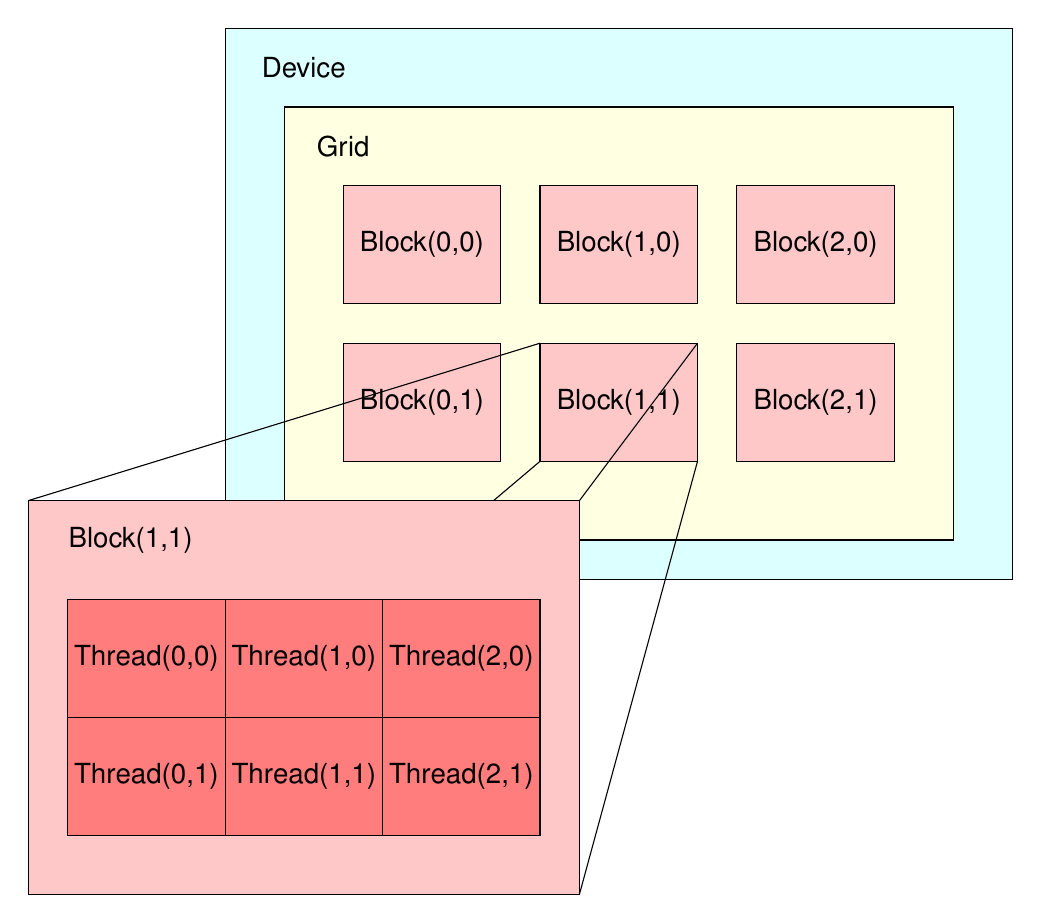
\begin{tikzpicture}
  % draw device rectangle
  \node at(0,0)[rectangle,draw,minimum width=10cm,minimum height=7cm,fill=devicecolor](device){};
  % draw "Device" text
  \node at(-4,3){\fontfamily{phv}\selectfont Device};
  % draw grid rectangle
  \node at(0,-.25)[rectangle,draw,minimum width=8.5cm,minimum height=5.5cm,fill=gridcolor](grid){};
  % draw "Grid" text
  \node at(-3.5,2){\fontfamily{phv}\selectfont Grid};
  % draw block rectangles inside grid rectangle
  \node at(-2.5,.75)[rectangle,draw,minimum width=2cm,minimum height=1.5cm,fill=blockcolor](block1){};
  \node at(0,.75)[rectangle,draw,minimum width=2cm,minimum height=1.5cm,fill=blockcolor](block2){};
  \node at(2.5,.75)[rectangle,draw,minimum width=2cm,minimum height=1.5cm,fill=blockcolor](block3){};
  \node at(-2.5,-1.25)[rectangle,draw,minimum width=2cm,minimum height=1.5cm,fill=blockcolor](block4){};
  \node at(0,-1.25)[rectangle,draw,minimum width=2cm,minimum height=1.5cm,fill=blockcolor](block5){};
  \node at(2.5,-1.25)[rectangle,draw,minimum width=2cm,minimum height=1.5cm,fill=blockcolor](block6){};
  % draw "Block(x,x)" text for each block
  \node at(-2.5,.75){\fontfamily{phv}\selectfont Block(0,0)};
  \node at(0,.75){\fontfamily{phv}\selectfont Block(1,0)};
  \node at(2.5,.75){\fontfamily{phv}\selectfont Block(2,0)};
  \node at(-2.5,-1.25){\fontfamily{phv}\selectfont Block(0,1)};
  \node at(0,-1.25){\fontfamily{phv}\selectfont Block(1,1)};
  \node at(2.5,-1.25){\fontfamily{phv}\selectfont Block(2,1)};
  % draw zoom lines to detailed block rectangle
  \draw (-1,-.5) -- (-7.5,-2.5);
  \draw (1,-.5) -- (-.5,-2.5);
  \draw (-1,-2) -- (-7.5,-7.5);
  \draw (1,-2) -- (-.5,-7.5);
  % draw detailed block rectangle
  \node at(-4,-5)[rectangle,draw,minimum width=7cm,minimum height=5cm,fill=blockcolor](detailedblock){};
  % draw "Block(1,1)" text for detailed block
  \node at(-6.2,-3){\fontfamily{phv}\selectfont Block(1,1)};
  % draw thread rectangles
  \node at(-6,-4.5)[rectangle,draw,minimum width=2cm,minimum height=1.5cm,fill=threadcolor](thread1){};
  \node at(-4,-4.5)[rectangle,draw,minimum width=2cm,minimum height=1.5cm,fill=threadcolor](thread2){};
  \node at(-2,-4.5)[rectangle,draw,minimum width=2cm,minimum height=1.5cm,fill=threadcolor](thread3){};
  \node at(-6,-6)[rectangle,draw,minimum width=2cm,minimum height=1.5cm,fill=threadcolor](thread4){};
  \node at(-4,-6)[rectangle,draw,minimum width=2cm,minimum height=1.5cm,fill=threadcolor](thread5){};
  \node at(-2,-6)[rectangle,draw,minimum width=2cm,minimum height=1.5cm,fill=threadcolor](thread6){};
  % draw "Thread(x,x)" text for each thread rectangle
  \node at(-6,-4.5){\smaller \fontfamily{phv}\selectfont Thread(0,0)};
  \node at(-4,-4.5){\smaller \fontfamily{phv}\selectfont Thread(1,0)};
  \node at(-2,-4.5){\smaller \fontfamily{phv}\selectfont Thread(2,0)};
  \node at(-6,-6){\smaller \fontfamily{phv}\selectfont Thread(0,1)};
  \node at(-4,-6){\smaller \fontfamily{phv}\selectfont Thread(1,1)};
  \node at(-2,-6){\smaller \fontfamily{phv}\selectfont Thread(2,1)};
\end{tikzpicture}
}
\caption{An overview of the CUDA programming model:}
\label{figure:background:graphical_processing_units:cuda-model}
\end{center}
\end{figure}
